\documentclass[12pt, a4paper, oneside]{Thesis} % Paper size, default font size and one-sided paper
\usepackage{wrapfig}
\usepackage{lscape}
\usepackage{rotating}
\usepackage{graphicx}
\usepackage{caption}
\usepackage{amsmath}


\usepackage{lineno,hyperref}
\modulolinenumbers[5]


\usepackage{amssymb}
\usepackage{graphicx}
\usepackage{array}
\usepackage{float}
\usepackage{placeins}
\usepackage{stackengine}
\usepackage{url}
\usepackage{numprint}
\usepackage{caption}

\usepackage{booktabs}  
\usepackage{siunitx}
\usepackage{subfigure}

\nprounddigits{3}
\newcolumntype{P}[1]{>{\centering\arraybackslash}p{#1}}
\newcolumntype{M}[1]{>{\centering\arraybackslash}m{#1}}

\setstackEOL{\#}
\setstackgap{L}{12pt}

\graphicspath{{Pictures/}} % Specifies the directory where pictures are stored
\usepackage[square,numbers]{natbib} % Use the natbib reference package - read up on this to edit the reference style; if you want text (e.g. Smith et al., 2012) for the in-text references (instead of numbers), remove 'numbers' v

\hypersetup{urlcolor=black, colorlinks=false} % Colors hyperlinks in blue - change to black if annoyingv`	

\thesistitle{Project Name }
\supervisor{Professor X}
\degree{Bachelor of Technology}
\degreemajor{[Department Name]}
\authors{Swaubhik Chakraborty}
\rollno{123456789}
\university{Central Institute of Technology}
\department{National Institute of Electronics \& Information Technology}
\unisite{https://www.cit.ac.in/}
\depsite{https://nielit.gov.in/guwahati/}
\placeshrt{Kokrajhar}
\placelng{Kokrajhar - 783370, India}
\datesub{\today}
\datesig{\today}
\semsub{Odd Semester, 2022-23}
\keywords{ML, IoT, Blockchain}
\coursecd{Industrial Training}
\subject{Machine Learning on Python}

\title{\ttitle} % Defines the thesis title - don't touch this
\begin{document}

\frontmatter 

\setstretch{1.6} % Line spacing of 1.6 (double line spacing)

% Define the page headers using the FancyHdr package and set up for one-sided printing
\fancyhead{} % Clears all page headers and footers
\rhead{\thepage} % Sets the right side header to show the page number
\lhead{} % Clears the left side page header

%\pagestyle{fancy} % Finally, use the "fancy" page style to implement the FancyHdr headers

\newcommand{\HRule}{\rule{\linewidth}{0.5mm}} % New command to make the lines in the title page

% PDF meta-data
\hypersetup{pdftitle={\ttitle}}
\hypersetup{pdfsubject=\subjectname}
\hypersetup{pdfauthor=\authornames}
\hypersetup{pdfkeywords=\keywordnames}

%----------------------------------------------------------------------------------------
%	TITLE PAGE
%----------------------------------------------------------------------------------------
\maketitle
%\titlepg % Add a gap in the Contents, for aesthetics

\clearpage % Start a new page

%----------------------------------------------------------------------------------------
%	DECLARATION PAGE
%	Your institution may give you a different text to place here
%----------------------------------------------------------------------------------------


\Declaration% Add a gap in the Contents, for aesthetics


%----------------------------------------------------------------------------------------
%	CERTIFICATE PAGE
%----------------------------------------------------------------------------------------

\addtotoc{Certificate} % Add the "Abstract" page entry to the Contents

\certificate{\addtocontents{toc}{}} % Add a gap in the Contents, for aesthetics

\clearpage % Start a new page

\certificateexam{\addtocontents{toc}{}}

\clearpage
%----------------------------------------------------------------------------------------
%	ABSTRACT PAGE
%----------------------------------------------------------------------------------------

\addtotoc{Abstract} % Add the "Abstract" page entry to the Contents

\abstract{\addtocontents{toc}{} % Add a gap in the Contents, for aesthetics

Enter content here. 
}

\clearpage % Start a new page



%----------------------------------------------------------------------------------------
%	ACKNOWLEDGEMENTS
%----------------------------------------------------------------------------------------

\setstretch{1.3} % Reset the line-spacing to 1.3 for body text (if it has changed)

\acknowledgements{\addtocontents{toc}{}%\vspace{1em}} % Add a gap in the Contents, for aesthetics

Enter acknowledgement content here.

}
\clearpage % Start a new page

%----------------------------------------------------------------------------------------
%	LIST OF CONTENTS/FIGURES/TABLES PAGES
%----------------------------------------------------------------------------------------

\pagestyle{fancy} % The page style headers have been "empty" all this time, now use the "fancy" headers as defined before to bring them back

\lhead{\emph{Contents}} % Set the left side page header to "Contents"
\tableofcontents % Write out the Table of Contents

\lhead{\emph{List of Figures}} % Set the left side page header to "List of Figures"
\listoffigures % Write out the List of Figures

\lhead{\emph{List of Tables}} % Set the left side page header to "List of Tables"
\listoftables % Write out the List of Tables

%----------------------------------------------------------------------------------------
%	ABBREVIATIONS
%----------------------------------------------------------------------------------------

\clearpage % Start a new page

\setstretch{1.5} % Set the line spacing to 1.5, this makes the following tables easier to read

\lhead{\emph{Abbreviations}} % Set the left side page header to "Abbreviations"
\listofsymbols{ll} % Include a list of Abbreviations (a table of two columns)
{
\textbf{CIT} & \textbf{C}entral \textbf{I}nstitute \textbf{T}echnology\\
\textbf{NIELIT} & \textbf{N}ational \textbf{I}nstitute of \textbf{E}lectronics \& \textbf{I}nformation \textbf{T}echnology\\
\textbf{FEA} & \textbf{F}inite \textbf{E}lement \textbf{A}nalysis \\
\textbf{FEM} & \textbf{F}inite \textbf{E}lement \textbf{M}ethod \\
\textbf{LVDT} & \textbf{L}inear \textbf{V}ariable \textbf{D}ifferential \textbf{T}ransformer \\
\textbf{RC} & \textbf{R}einforced \textbf{C}oncrete
%\textbf{Acronym} & \textbf{W}hat (it) \textbf{S}tands \textbf{F}or \\
}

%----------------------------------------------------------------------------------------
%	SYMBOLS
%----------------------------------------------------------------------------------------

\clearpage % Start a new page

\lhead{\emph{Symbols}} % Set the left side page header to "Symbols"

\listofnomenclature{lll} % Include a list of Symbols (a two column table)
{
$D^{el}$ & elasticity tensor \\
$\sigma$ & stress tensor \\
$ \varepsilon $ & strain tensor \\
% Symbol & Name & Unit \\

}

%----------------------------------------------------------------------------------------
%	THESIS CONTENT - CHAPTERS
%----------------------------------------------------------------------------------------

\mainmatter % Begin numeric (1,2,3...) page numbering

\pagestyle{fancy} % Return the page headers back to the "fancy" style

% Include the chapters of the thesis as separate files from the Chapters folder
% Uncomment the lines as you write the chapters

% Chapter Template

\chapter{Introduction to Summer Internship} % Main chapter title
\graphicspath{{Pictures/Chapter1}}
\label{Chapter 1} % Change X to a consecutive number; for referencing this chapter elsewhere, use \ref{ChapterX}

\lhead{Chapter 1. \emph{Introduction to Summer Internship}} % Change X to a consecutive number; this is for the header on each page - perhaps a shortened title

%----------------------------------------------------------------------------------------
%	SECTION 1
%---------------------------------------------------------------------------------------
\section{CITK}
The Central Institute of Technology Kokrajhar (CITK) is a public technical university established in 2006 and owned by the Government of India. It is located in Kokrajhar, Assam, India. The institute is spread across 300 acres (1.2 km2) in Kokrajhar and offers Bachelor of Technology (B.Tech.), Bachelor of Design (B.Des.), Master of Technology (M.Tech.), Master of Design (M.Des.),Doctor of Philosophy (PhD), and Diploma programs in various disciplines.\cite{enwiki:citk}
%----------------------------------------------------------------------------------------
%	SECTION 2
%---------------------------------------------------------------------------------------
\section{NIELIT Guwahati}
National Institute of Electronics \& Information Technology (NIELIT), formerly known as the DOEACC Society, is a society that offers Information Technology and Electronics training at different levels.

\begin{figure}[!htbp]
\centering
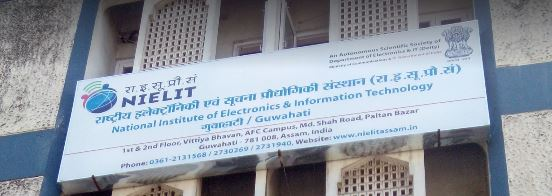
\includegraphics[width=15cm]{nielit.jpeg}
\caption{NIELIT Guwahati}
\label{fignielit}
\end{figure}

It is associated with the Ministry of Electronics and Information Technology of the Government of India.\cite{enwiki:nielit} \par

NIELIT Guwahati is located at 1st \& 2nd floor, Vittiya Bhavan,AFC Building, Md. Shah Road Paltan Bazar, Guwahati - 781008, ASSAM Phone:- 0361-2730269

%----------------------------------------------------------------------------------------
%	SECTION 3
%---------------------------------------------------------------------------------------
\section{About Training}
Here is a detailed overview of our summer internship experience, highlighting the day-to-day activities and tasks accomplished during the internship period. The internship provided valuable opportunities to gain practical knowledge, enhance skills, and apply academic learning in a professional setting. This report aims to provide a comprehensive summary of our internship experience on Machine Learning using Python.

Duration: 20-June-2023 to 20-July-2023

\textbf{Day 1}
\begin{itemize}
    \item Orientation program, including an overview of the internship program, expectations, and guidelines
    \item Meeting the supervisor and discussing the internship objectives and project details.
    \item Introduction to Git and GitHub
\end{itemize}

\textbf{Day 2-5}
\begin{itemize}
    \item Introduction to python (Data types, conditions statements, loops)
    \item Introduction to python Libraries (Numpy, Pandas)
    \item Hands-on session on Numpy \& Pandas.
    \item Introduction to Visualization Libraries (Matplotlib, Seaborn) using Iris Dataset
    \item Introduction to Machine Learning \& Types of Machine Learning
    \item Hands-on Machine Learning
\end{itemize}

\textbf{Day 6-10}
\begin{itemize}
    \item Introduction to Neural Networks \& Other optimization algorithms
    \item Introduction to Backpropagation algorithm
    \item Activation functions, Hyper-parameters, Dataset processing
    \item Introduction to Keras/Tensorflow (Hands-on)
    \item Introduction to Convolutional Neural Networks 
   
\end{itemize}
\textbf{Day 11-15}
\begin{itemize}
    \item Activation functions, Hyper-parameters, Dataset processing 
    \item Implementation of flower classification problem in Keras (Hands-on)
    \item Data augmentation (Hands-on using Flower Classification problem)
    \item Pre-trained Models - AlexNet, ResNet, DenseNet in Keras, Transfer learning. AlexNet and Implementation of AlexNet in Keras
    \item Implementation of ResNet, DenseNet in Keras (Hands-on)
\end{itemize}
\textbf{Day 16-20}
\begin{itemize}
    \item Introduction to Recurrent Neural Networks
    \item Introduction to Long Short Term Memory (LSTM)
    \item Sequence Modelling
    \item Data Cleaning and Preprocessing for NLP
    \item Transformers (Attention is all you need)
    \item Implementation of Transformers - Walk through \& Hands-on 
    \item Model deployment on web application and MLOps (Hands-on Python and Flask)
\end{itemize}
\textbf{Day 20-25}
\begin{itemize}
    \item Started working of Project
    \item Doubt sessions
    \item Mentoring Sessions
\end{itemize}
\input{Chapters/Chapter2} 
%\input{Chapters/Chapter5} 
%\input{Chapters/Chapter6} 
%\input{Chapters/Chapter7} 

%----------------------------------------------------------------------------------------
%	THESIS CONTENT - APPENDICES
%----------------------------------------------------------------------------------------

\addtocontents{toc}{\vspace{2em}} % Add a gap in the Contents, for aesthetics

\appendix % Cue to tell LaTeX that the following 'chapters' are Appendices

% Include the appendices of the thesis as separate files from the Appendices folder
% Uncomment the lines as you write the Appendices

\input{Appendices/AppendixA}
%\input{Appendices/AppendixB}
%\input{Appendices/AppendixC}

\addtocontents{toc}{} % Add a gap in the Contents, for aesthetics

\backmatter

%----------------------------------------------------------------------------------------
%	BIBLIOGRAPHY
%----------------------------------------------------------------------------------------
%\nocite{*}
\label{Bibliography}

\lhead{\emph{Bibliography}} % Change the page header to say "Bibliography"

\bibliographystyle{apalike} % Use the "custom" BibTeX style for formatting the Bibliography

\bibliography{Bibliography} % The references (bibliography) information are stored in the file named "Bibliography.bib"

\end{document}  
